\documentclass[10pt,a4paper]{article}

% ─── Packages ─────────────────────────────────────────

\usepackage{fontspec}
\setmainfont{Times New Roman}

\usepackage[top=0.6cm,bottom=0.5cm,left=1.45cm,right=1.45cm]{geometry}

\usepackage{titlesec}
\usepackage{enumitem}
\usepackage{hyperref}
\usepackage{xcolor}
\usepackage{tabularx}
\usepackage{graphicx}
\usepackage{parskip}

% ─── Colors ───────────────────────────────────────────

\definecolor{primary}{RGB}{30,40,90}
\definecolor{namecolor}{RGB}{0,120,180}
\definecolor{accent}{RGB}{50,90,150}
\definecolor{rulecol}{RGB}{200,205,220}
\definecolor{gray}{RGB}{90,90,90}

\hypersetup{
    colorlinks=true,
    urlcolor=accent
}

\pagestyle{empty}
\setlength{\parskip}{0pt}

% ─── Section ──────────────────────────────────────────

\titleformat{\section}
    {\normalsize\bfseries\color{primary}}
    {}
    {0em}
    {}
    [\vspace{1pt}\textcolor{rulecol}{\titlerule[0.6pt]}\vspace{1pt}]

\titlespacing{\section}{0pt}{3pt}{1pt}

% ─── Entry ────────────────────────────────────────────

\newcommand{\entry}[3]{%
    \noindent
    \begin{tabularx}{\linewidth}{X r}
        \textbf{\color{primary}#1} &
        {\scriptsize\color{gray}#2}
    \end{tabularx}\\[-2pt]
    {\scriptsize\textit{\color{gray}#3}}
    \vspace{0.5pt}
}

% ─── Compact list ─────────────────────────────────────

\newenvironment{cvitems}{
    \begin{itemize}[
        leftmargin=1.1em,
        topsep=0pt,
        itemsep=0.3pt,
        parsep=0pt,
        partopsep=0pt
    ]
}{
    \end{itemize}
}

% ═════════════════════════════════════════════════════

\begin{document}

% ─── HEADER ───────────────────────────────────────────

\noindent

\begin{tabularx}{\linewidth}{@{}X r@{}}

\begin{minipage}[c]{\linewidth}

    {\LARGE\bfseries\color{namecolor} Ho Huynh Nhu}\\[1pt]

    {\large\bfseries\color{primary}
    Business Analyst Intern}\\[2pt]

    {\scriptsize\color{gray}
    20/10/2003
    \enspace\textcolor{rulecol}{|}
    \enspace (+84) 367 503 477
    \enspace\textcolor{rulecol}{|}
    \enspace
    \href{mailto:hhnhu2003@gmail.com}{hhnhu2003@gmail.com}
    \enspace\textcolor{rulecol}{|}
    \enspace Ho Chi Minh City}\\[1pt]

    {\scriptsize
    \href{https://github.com/hohuynhnhu}
    {github.com/hohuynhnhu}
    \enspace\textcolor{rulecol}{|}
    \enspace
    \href{https://www.facebook.com/huynhnhu.ho.961}
    {facebook.com/huynhnhu.ho.961}
    }

\end{minipage}

&

\begin{minipage}[c]{2.1cm}
    \raggedleft
    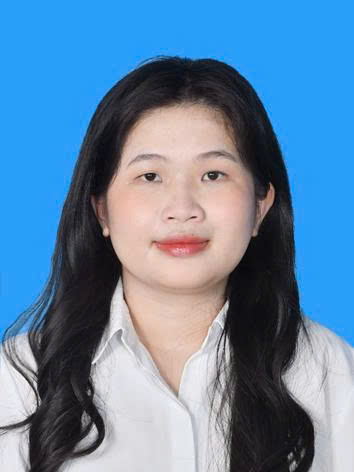
\includegraphics[
        width=2.1cm,
        height=2.5cm,
        keepaspectratio
    ]{assets/avt.jpg}
\end{minipage}

\end{tabularx}

\vspace{1pt}

\textcolor{rulecol}{\rule{\linewidth}{0.6pt}}

% ─── CAREER OBJECTIVE ─────────────────────────────────

\section*{Career Objective}

{\small
Final-year IT student with hands-on experience in SQL, Excel, data
analysis and Power BI, and practical exposure to gathering
requirements, cleaning data, and building reports that support
business decisions. Comfortable working with stakeholders to
understand processes and turn data into actionable insight. Seeking
a Business Analyst internship to grow into business process analysis
and the Microsoft Power Platform (Power Apps, Power Automate,
Dataverse).
}

% ─── EDUCATION ────────────────────────────────────────

\section*{Education}

\entry
{University of Transport Ho Chi Minh City (UTH)}
{10/2022 -- 10/2026}
{Bachelor of Information Technology -- Completed coursework}

{\small
\begin{cvitems}

    \item GPA: \textbf{3.4 / 4.0}

    \item \textbf{Excellent Scholarship} -- Semester 1, 2025

    \item \textbf{Second Prize -- AI Track},
    UTH Student Scientific Research Conference 2025

\end{cvitems}
}

% ─── TECHNICAL SKILLS ─────────────────────────────────

\section*{Skills}

{\small

\begin{tabularx}{\linewidth}{@{}lX@{}}

\textbf{Business Analysis}
&
Requirements Gathering, Stakeholder Communication, As-Is/To-Be Process
Analysis, Process Documentation, KPI Definition, UAT Support
\\[1pt]

\textbf{Data \& Reporting}
&
Data Cleaning, Data Transformation, Data Validation, Exploratory Data
Analysis, Trend Analysis, Operational Reporting
\\[1pt]

\textbf{SQL}
&
SQL, PostgreSQL, SQL Server, MySQL, Joins, CTEs, Aggregations,
Subqueries, Window Functions
\\[1pt]

\textbf{BI / Visualization}
&
Power BI, DAX, Dashboard Development, Data Visualization
\\[1pt]

\textbf{Excel}
&
Data Cleaning, Data Filtering, Pivot Tables, Lookup Functions, Reporting
\\[1pt]

\textbf{Python}
&
Python, Pandas, NumPy, Data Processing Automation
\\[1pt]

\textbf{ETL / Data}
&
ETL/ELT, dbt, Apache Airflow, Data Pipeline, Data Modeling
\\[1pt]

\textbf{Databases}
&
PostgreSQL, SQL Server, MySQL, MongoDB, Firebase, Supabase
\\[1pt]

\textbf{Tools}
&
Git, Docker, Postman, VS Code, Jira, Confluence
\\[1pt]

\textbf{Currently Learning}
&
Power Platform fundamentals (Power Apps, Power Automate, Dataverse)

\end{tabularx}

}

% ─── WORK EXPERIENCE ──────────────────────────────────

\section*{Work Experience}

\entry
{Gotik Consulting -- Data Engineer}
{Python \textbar{} dbt \textbar{} PostgreSQL \textbar{} Airflow \textbar{} Power BI}
{03/2026 -- 05/2026}

{\small
\begin{cvitems}
    \item Worked with business data owners to understand Odoo business
    processes and requirements, then documented and translated them
    into clean, structured datasets for analytics and reporting.

    \item Built Python-based ETL pipelines and dbt models to extract,
    clean, and structure raw data into reusable analytical datasets in
    Neon PostgreSQL, with hourly workflows automated in Apache Airflow.

    \item Gathered reporting requirements and KPIs from stakeholders
    and built Power BI dashboards to support monitoring and
    data-driven decision-making.

    \item Wrote SQL queries for aggregation, filtering, and joins to
    ensure reliable, analysis-ready data sources for downstream
    reports.
\end{cvitems}
}

% ─── PROJECTS ─────────────────────────────────────────

\section*{Featured Projects}

\entry
{Delivery Driver -- Order Analytics System}
{Python \textbar{} SQL \textbar{} Kafka \textbar{} PostgreSQL \textbar{} Power BI}
{12/2025 -- 02/2026}

{\small
\begin{cvitems}
    \item Gathered and analyzed requirements for order data reporting;
    built a Data Lake / Data Warehouse pipeline to prepare data for
    analysis.
    \item Applied RFM and Association Rule Mining to analyze customer
    behavior and surface frequent pickup--delivery patterns for
    business use.
    \item GitHub: \href{https://github.com/LeKhang-cn22h/BE-delivery-driver}{BE-delivery-driver}
\end{cvitems}
}

\vspace{1pt}

\entry
{VehicleScan -- Smart Parking Data System}
{Python \textbar{} SQL \textbar{} PostgreSQL \textbar{} Firebase \textbar{} ESP32}
{03/2025 -- 03/2026}

{\small
\begin{cvitems}
    \item Analyzed operational requirements for a real-time parking
    monitoring use case and processed vehicle/IoT sensor data using
    Python and SQL.
    \item Integrated AI, sensor, and application data into a
    centralized system to support monitoring and reporting.
    \item GitHub: \href{https://github.com/LeKhang-cn22h/VehicleScanner}{VehicleScanner}
\end{cvitems}
}

% ─── ADDITIONAL INFORMATION ───────────────────────────

\section*{Additional Information}

{\small

\begin{tabularx}{\linewidth}{@{}lX@{}}

\textbf{English}
&
Technical document reading and basic professional communication

\\[1pt]

\textbf{Availability}
&
Available for a full-time or part-time Business Analyst internship

\end{tabularx}

}
\end{document}